\section{C\'ordoba sector square function on $\R^{2}$}

We begin with a square function inequality for Fourier multipliers adapted to a collection of \emph{congruent} finitely overlapping rectangles of fixed orientation in $\R^{n}$.
In \cite{MR850681} this result is attributed to Carleson (in dimension $n=1$, although the higher-dimensional case does not present additional difficulties).
There is also an alternative proof by C\'ordoba \cite{MR639467} that I have not looked up.

There are also bounds for square functions associated to \emph{arbitrary} finitely overlapping rectangles of fixed orientation.
In dimension $n=1$ it is due to Rubio de Francia \cite{MR850681}, and in higher dimensions to Lacey \cite{MR2293255}.
We will not need such general results.

\begin{lemma}
\label{lem:pointwise-square-bound}
For every $n\in\N$ and $N>0$ there exists $M<\infty$ such that the following holds.
Let $\Xi$ be a $1$-separated set in $\R^{n}$ and for each $\xi\in\Xi$ let $\phi_{\xi}$ be a Schwartz function with $M$-th Schwartz norm bounded by $1$.
Then
\begin{equation}
\label{eq:pointwise-square-bound}
\sum_{\xi\in\Xi} \abs[\Big]{ \int_{\R^{n}} \phi_{\xi}(x) f(x) e(x\cdot \xi) \dif x }^{2}
\lesssim_{n,N}
\int_{\R^{n}} \abs{f(x)}^{2} (1+\abs{x})^{-N} \dif x.
\end{equation}
\end{lemma}
\begin{proof}
By Plancherel's theorem it is easy to obtain the estimate \eqref{eq:pointwise-square-bound} with $N=0$.
To pass to larger $N$ split the domain of $f$ into a ball of radius $1$ and dyadic shells of radii $R\in 2^{\N}$.
For a dyadic shell of radius $R$ let $\chi_{R}$ be a smooth approximation of its characteristic function.
Then, for $C=C(M,N)$ large enough,
\[
\norm{ \chi_{R}\phi }_{M-\mathrm{Schwartz}}
\lesssim
R^{-10 N} \norm{ \chi_{R}\phi }_{(M+C)-\mathrm{Schwartz}}.
\]
Hence we can sum up the contributions of the dyadic shells.
\end{proof}
\begin{corollary}
\label{lem:square-fct-congruent-cubes}
Let $\calQ$ be a boundedly overlapping collection of unit cubes in $\R^{n}$.
For each $Q\in\calQ$ let $m_{Q}$ be a bump function adapted to $Q$ (with sufficiently many derivatives depending on $n$).
Then for $2 \leq p \leq \infty$ we have
\[
\norm[\Big]{ \Bigl( \sum_{Q\in\calQ} \abs{\calF^{-1}(m_{Q} \hat{f})}^{2} \Bigr)^{1/2} }_{L^{p}(\R^{n})}
\lesssim
\norm{ f }_{L^{p}(\R^{n})}.
\]
\end{corollary}
By scaling and rotation invariance we can replace $\calQ$ by a collection of rectangles of any fixed size with sides parallel to some coordinate axes.
\begin{proof}
Let $w \in L^{(p/2)'}(\R^{n})$.
Applying Lemma~\ref{lem:pointwise-square-bound} to the shifted function $f(x-\cdot)$ we obtain
\[
\sum_{Q\in\calQ} \abs{\calF^{-1}(m_{Q} \hat{f})(x)}^{2}
\lesssim
\int_{\R^{n}} \abs{f(x-y)}^{2} (1+\abs{y})^{-N} \dif y
\]
for some $N>n$ provided that we assume sufficiently many derivative bounds on $m_{Q}$'s.
Multiplying this inequality by $w(x)$ and integrating in $x$ we obtain
\begin{multline*}
\int_{\R^{n}} \sum_{Q\in\calQ} \abs{\calF^{-1}(m_{Q} \hat{f})(x)}^{2} w(x) \dif x
\lesssim
\int_{\R^{n}} \int_{\R^{n}} \abs{f(x-y)}^{2} (1+\abs{y})^{-N} \dif y w(x) \dif x\\
=
\int_{\R^{n}} \abs{f(x)}^{2} \bigl( w * (1+\abs{\cdot})^{-N} \bigr)(x) \dif x\\
\leq
\norm{f}_{p}^{2} \norm{ w * (1+\abs{\cdot})^{-N} }_{(p/2)'}
\lesssim
\norm{f}_{p}^{2} \norm{ w }_{(p/2)'}.
\end{multline*}
Taking the supremum over all $w$ with $\norm{ w }_{(p/2)'}=1$ and using duality we obtain the claim.
\end{proof}

\begin{remark}
Square function inequalities for \emph{arbitrary} collections of cubes \cite{MR850681,MR2293255} hold only in the range $2\leq p<\infty$.
A heuristic explanation for this smaller range is that instead of the convolution of $w$ with a fixed function we would see convolutions with varying functions, so we would need to estimate some maximal function of $w$, which is not possible for $p=\infty$ since in this case $(p/2)'=1$.
We emphasize however that the above proof in inadequate for more general collections of rectangles.
\end{remark}

\begin{center}
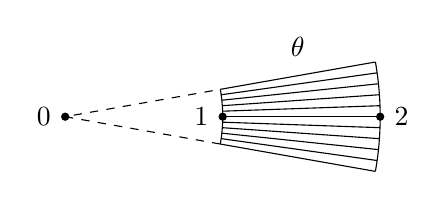
\begin{tikzpicture}[scale=2]
\node[circle,fill=black,inner sep=0pt,minimum size=3pt,label=left:{$0$}] at (0,0) {};
\node[circle,fill=black,inner sep=0pt,minimum size=3pt,label=left:{$1$}] at (1,0) {};
\node[circle,fill=black,inner sep=0pt,minimum size=3pt,label=right:{$2$}] at (2,0) {};
\draw (0,0) +(-10:1) arc (-10:10:1);
\draw (0,0) +(-10:2) arc (-10:10:2);
\foreach \a in {-10,-8,...,10}
{
  \draw (\a:1) -- (\a:2);
}
\draw[dashed] (-10:1) -- (0,0) -- (10:1);
\node[label=above:{$\theta$}] at (10:1.5) {};
\end{tikzpicture}
\end{center}

\begin{proposition}
Let $\theta$ be a collection of disjoint truncated sectors of angle $\sim 1/N$ as in the figure.
For each $\theta$ let $P_{\theta}$ be a smooth Fourier multiplier operator adapted to $\theta$.
Then
\begin{equation}
\label{eq:cordoba-sq-fct:annulus}
L^{4} \ell^{2}_{\theta} \abs{P_{\theta} * f}
\lesssim
(\log N)^{1/4}
L^{4} f.
\end{equation}
\end{proposition}
\begin{proof}
Expanding the $4$-th power of the left-hand side of \eqref{eq:cordoba-sq-fct:annulus} we obtain
\[
\int_{\R^{2}} \sum_{\theta,\theta'} \abs{P_{\theta}f}^{2} \abs{P_{\theta'}f}^{2}.
\]
We split the summation
\[
\sum_{m=0}^{\log_{2} N} \sum_{\theta,\theta' : \dist(\theta,\theta') \sim 2^{-m}} \int_{\R^{2}} \abs{P_{\theta}f}^{2} \abs{P_{\theta'}f}^{2}.
\]
It suffices to obtain a uniform (in $N$) bound for each $m$-summand.
All estimates below will be uniform in $N$.

For the diagonal term $\theta=\theta'$ we obtain an $L^{4} \to L^{4}\ell^{4}$ estimate by interpolation between the $L^{2}\to L^{2}\ell^{2}$ estimate which follows from Plancherel's theorem and the trivial $L^{\infty} \to L^{\infty}\ell^{\infty}$ estimate.

Now fix $m$ and partition each $\theta$ in pieces $\theta_{\alpha}$, $\alpha = 1,\dotsc,CN/2^{m}$, of size $1/N \times 2^{m}/N$.
Split $P_{\theta} = \sum_{\alpha} P_{\theta,\alpha}$ accordingly (each piece is a smooth multiplier).
\begin{center}
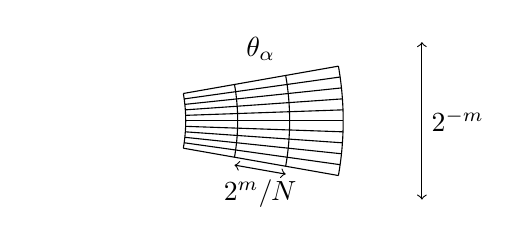
\begin{tikzpicture}[scale=2]
\draw (0,0) +(-10:1) arc (-10:10:1);
\draw (0,0) +(-10:1.33) arc (-10:10:1.33);
\draw (0,0) +(-10:1.66) arc (-10:10:1.66);
\draw (0,0) +(-10:2) arc (-10:10:2);
\foreach \a in {-10,-8,...,10}
{
  \draw (\a:1) -- (\a:2);
}
\node[label=above:{$\theta_{\alpha}$}] at (10:1.5) {};
\begin{scope}[yshift=-0.05cm]
\draw[<->] (-10:1.33) -- (-10:1.66) node [midway, below] {$2^{m}/N$};
\end{scope}
\draw[<->] (2.5,-0.5) -- (2.5,0.5) node [midway, right] {$2^{-m}$};
\end{tikzpicture}
\end{center}
For $\theta,\theta'$ with angular distance $\sim 2^{-m}$ the sumsets $\theta_{\alpha}+\theta'_{\beta}$ have bounded overlap as $\alpha,\beta$ vary.
Hence
\begin{multline*}
\sum_{\theta,\theta' : \dist(\theta,\theta') \sim 2^{-m}} \int_{\R^{2}} \abs{P_{\theta}f}^{2} \abs{P_{\theta'}f}^{2}
=
\sum_{\theta,\theta' : \dist(\theta,\theta') \sim 2^{-m}} \int_{\R^{2}} \abs{\sum_{\alpha,\beta} P_{\theta,\alpha}f P_{\theta',\beta}f}^{2}\\
\lesssim
\sum_{\theta,\theta' : \dist(\theta,\theta') \sim 2^{-m}} \sum_{\alpha,\beta} \int_{\R^{2}} \abs{P_{\theta,\alpha}f P_{\theta',\beta}f}^{2}.
\end{multline*}
We split the sum over $\theta$ into pieces with $\sim N/2^{m}$ consecutive summands.
For each piece denote by $\Theta$ the set of all $\theta$ and $\theta'$ that give nontrivial contribution, then each $\Theta$ contains $\sim N/2^{m}$ consecutive summands and $\Theta$'s have bounded overlap.
We estimate the previous display by
\[
\leq
\sum_{\Theta} \sum_{\theta,\theta' \in \Theta} \sum_{\alpha,\beta} \int_{\R^{2}} \abs{P_{\theta,\alpha}f P_{\theta',\beta}f}^{2}
=
\sum_{\Theta} \int_{\R^{2}} \Bigl( \sum_{\theta \in \Theta} \sum_{\alpha} \abs{P_{\theta,\alpha}f}^{2} \Bigr)^{2},
\]
By the already mentioned $L^{4} \to L^{4}\ell^{4}$ bound it suffices to consider each $\Theta$ individually.
Now for fixed $\Theta$ all sectors $\theta_{\alpha}$, $\theta \in \Theta$, are comparable to rectangular boxes of size $\sim 1/N \times 2^{m}/N$ of a \emph{fixed orientation}.
To see this assume without loss of generality that the sectors in $\Theta$ are close to horizontal.
Then rescale them by a factor $2^{-m}$ in the horizontal direction.
After rescaling the slopes of all sectors $\theta_{\alpha}$ are still $\lesssim 1$, and both their width and height become $\sim 1/N$.
Hence we can apply a suitably rescaled version of Corollary~\ref{lem:square-fct-congruent-cubes}.
\end{proof}

\begin{remark}
The truncation of the sectors can be removed as shown in \cite{MR688026,MR730074} at the cost of another power of $\log N$.
It is also possible to replace the smooth Fourier multipliers by sharp Fourier cutoffs.
To this end one can use the so-called Meyer vector-valued inequality
\begin{equation}
\label{eq:Meyer-directional-ineq}
L^{4} \ell^{2}_{j,l} \abs{T_{j} f_{j,l}}
\lesssim
(\log N)^{C} L^{4} \ell^{2}_{j,l} \abs{f_{j,l}},
\end{equation}
where $T_{j}$, $j=1,\dotsc,N$, are Hilbert transforms along $1/N$-separated directions in $\R^{2}$.
The inequality \eqref{eq:Meyer-directional-ineq} was first proved in \cite{MR0438022} using a weighted inequality for the Hilbert transform and bounds for a directional maximal operator in $\R^{2}$.
Since the separation hypothesis for directional maximal operators was later removed by Katz \cite{MR1681088}, this approach also yields \eqref{eq:Meyer-directional-ineq} with an arbitrary set of $N$ directions.

In \cite[Section 8.2]{arxiv:1902.03644} it is worked out that the weighted approach, when paired with sharp weighted estimates for the Hilbert transform, gives \eqref{eq:Meyer-directional-ineq} with bound $(\log N)^{1}$.

The article \cite{arxiv:1902.03644} also provides an alternative approach to estimates such as \eqref{eq:cordoba-sq-fct:annulus} and \eqref{eq:Meyer-directional-ineq}.
\end{remark}

%%% Local Variables:
%%% mode: latex
%%% TeX-master: decoupling-notes
%%% End:
